%%%%%%%%%%%%%%%%%%%%%%%%%%%%%%%%%%%%%%%%%%%%%%%%%%%%%%%%%%%%%%%%%
%%%%%%%%%%%%%%%%%%%%%%%%%%%%%%%%%%%%%%%%%%%%%%%%%%%%%%%%%%%%%%%%%
\setcounter{chapter}{4}
\newcommand{\graphicscompanion}{\emph{The \LaTeX{} Graphics Companion}~\cite{graphicscompanion}} 
\newcommand{\hobby}{\emph{A User's Manual for MetaPost}~\cite{metapost}}
\newcommand{\hoenig}{\emph{\TeX{} Unbound}~\cite{unbound}}
\newcommand{\graphicsinlatex}{\emph{Graphics in \LaTeXe{}}~\cite{ursoswald}}

\chapter{Producción de gráficos matemáticos}
\label{chap:graphics}

\begin{intro}
Mucha gente usa \LaTeX\ para componer sus textos; pero además del enfoque orientado a la estructura (y no al contenido) tan conveniente, \LaTeX\ también ofrece la posibilidad (si bien bastante restringida) de producir salidas gráficas a partir de descripciones textuales.  Por otro lado, se han creado varias extensiones de  \LaTeX\ para evadir estas restricciones.  En esta sección aprenderá algunas de ellas.
\end{intro}

\section{Panorama general}

El entorno \ei{picture} permite programar dibujos directamente en \LaTeX.  Una descripción detallada puede encontrarse en el \manual. Por un lado hay restricciones serias, como que las pendientes de los segmentos de recta así como los radios de los círculos están restringidos a un número corto de valores.  Por otro lado, el entorno \ei{picture} de \LaTeXe\ trae con él la orden \ci{qbezier}, donde ``\texttt{q}'' significa ``cuadrática''.  Muchas curvas usadas con frecuencia, como círculos, elipses o catenarias, puedes aproximarse satisfactoriamente con curvas de  B\'ezier cuadráticas, aunque esto puede requerir algo de matemáticas.  Si además se utiliza un lenguaje de programación como Lisp para generar bloques \ci{qbezier} de \filenomo{}s de entrada \LaTeX, el entorno \ei{picture} se vuelve bastante potente.

Aunque la programación de dibujos directamente en  \LaTeX\ tiene muchas
restricciones, y es a menudo muy incómodo, puede haber razones para hacerlo. Los documentos producidos son ``pequeños'' en cuanto al tamaño en octetos, y no hay que andar  arrastrando \filenomo{}s gráficos adicionales.

Los paqueteos como \pai{epic} y \pai{eepic} (descritos, por ejemplo, en \companion) o \pai{pstricks} ayudan a eliminar las restricciones a las que está sujeto el entorno \ei{picture} original, y refuerzan en gran medida la potencia gráfica de \LaTeX.

Mientras los dos primeros paquetes sólo mejoran el entorno \ei{picture}, el paquete \pai{pstricks} tiene sus propio entorno de dibujo, \ei{pspicture}.  La potencia de  \pai{pstricks} se basa en el hecho de que este paquete hace uso extenso de las posibilidades de \PSi{}.  Además, numerosos paquetes han sido escritos para propósitos específicos.  Uno de ellos es \texorpdfstring{\Xy}{Xy}-pic, descrito al final de este capítulo.  Una amplia variedad de estos paquetes se describe en detalle en \graphicscompanion{} (no lo confunda con \companion).

Quizás la herramienta gráfica más potente relacionada con \LaTeX\ es
\texttt{MetaPost}, el gemelo de \texttt{METAFONT} de Donald E. Knuth. \texttt{MetaPost} tiene el lenguaje de programación de \texttt{METAFONT}, muy potente y matemáticamente sofisticado; pero al contrario que \texttt{METAFONT}, que genera mapas de pixeles, \texttt{MetaPost} genera \filenomo{}s de Encapsulated \PSi{}, que pueden importarse en \LaTeX.  Para una introducción, vea \hobby, o el tutorial de \cite{ursoswald}.

Una discusión minuciosa sobre estrategias en \LaTeX{} y \TeX{} para gráficos (y \fontsnomo{}) puede encontrarse en \hoenig.

\section{El entorno \texttt{picture}}
\secby{Urs Oswald}{osurs@bluewin.ch}

\subsection{Órdenes básicas}

Se crea un entorno \ei{picture}\footnote{Lo crea o no, el entorno picture funciona sin más, con \LaTeXe{} normal, sin necesidad de cargar ningún paquete.} con alguna de las dos órdenes
\begin{lscommand}
\ci{begin}\verb|{picture}(|$x,y$\verb|)|\ldots\ci{end}\verb|{picture}|
\end{lscommand}
o
\begin{lscommand}
\ci{begin}\verb|{picture}(|$x,y$\verb|)(|$x_0,y_0$\verb|)|\ldots\ci{end}\verb|{picture}|
\end{lscommand}
Los números $x,\,y,\,x_0,\,y_0$ se refieren a \ci{unitlength}, que
puede establecerse en cualquier momento
(pero no dentro de un entorno \ei{picture}) con una orden como
\begin{lscommand}
\ci{setlength}\verb|{|\ci{unitlength}\verb|}{1.2cm}|
\end{lscommand}
El valor por omisión de \ci{unitlength} es \texttt{1pt}.  El primer par, $(x,y)$, reserva dentro del documento un espacio rectangular para el dibujo.  El segundo par, opcional, $(x_0,y_0)$, asigna coordenadas arbitrarias a la esquina inferior izquierda del rectángulo reservado.

La mayoría de las órdenes de dibujo tienen alguna de las dos formas
\begin{lscommand}
\ci{put}\verb|(|$x,y$\verb|){|\emph{objeto}\verb|}|
\end{lscommand}
o
\begin{lscommand}
\ci{multiput}\verb|(|$x,y$\verb|)(|$\Delta x,\Delta
y$\verb|){|$n$\verb|}{|\emph{objeto}\verb|}|\end{lscommand}
Las curvas de B\'ezier son una excepción.  Se dibujan con la orden
\begin{lscommand}
\ci{qbezier}\verb|(|$x_1,y_1$\verb|)(|$x_2,y_2$\verb|)(|$x_3,y_3$\verb|)|
\end{lscommand}
\newpage

\subsection{Segmentos de recta}
\begin{example}
\setlength{\unitlength}{5cm}
\begin{picture}(1,1)
  \put(0,0){\line(0,1){1}}
  \put(0,0){\line(1,0){1}}  
  \put(0,0){\line(1,1){1}}  
  \put(0,0){\line(1,2){.5}}
  \put(0,0){\line(1,3){.3333}}
  \put(0,0){\line(1,4){.25}}  
  \put(0,0){\line(1,5){.2}}
  \put(0,0){\line(1,6){.1667}}
  \put(0,0){\line(2,1){1}}
  \put(0,0){\line(2,3){.6667}}
  \put(0,0){\line(2,5){.4}}
  \put(0,0){\line(3,1){1}}  
  \put(0,0){\line(3,2){1}}
  \put(0,0){\line(3,4){.75}}
  \put(0,0){\line(3,5){.6}}
  \put(0,0){\line(4,1){1}}
  \put(0,0){\line(4,3){1}}  
  \put(0,0){\line(4,5){.8}}
  \put(0,0){\line(5,1){1}}
  \put(0,0){\line(5,2){1}}
  \put(0,0){\line(5,3){1}}
  \put(0,0){\line(5,4){1}}
  \put(0,0){\line(5,6){.8333}}
  \put(0,0){\line(6,1){1}}
  \put(0,0){\line(6,5){1}}
\end{picture}
\end{example}
Se dibujan segmentos de recta con la orden
\begin{lscommand}
\ci{put}\verb|(|$x,y$\verb|){|\ci{line}\verb|(|$x_1,y_1$\verb|){|$length$\verb|}}|
\end{lscommand}
La orden \ci{line} tiene dos argumentos:
\begin{enumerate}
  \item un vector director,
  \item una longitud.
\end{enumerate}
Los componentes del vector director están restringidos a los enteros
\[-6,\,-5,\,\ldots,\,5,\,6, \] y tienen que ser primos entre sí (coprimos; sin divisor común salvo 1).  La figura ilustra los 25 posibles valores de las pendientes en el primer cuadrante.  La longitud es relativa a \ci{unitlength}.  El argumento longitud es la coordenada vertical en el caso de un segmento de recta vertical; el el resto de los casos, la coordenada horizontal.

\subsection{Flechas}

\begin{example}
\setlength{\unitlength}{0.75mm}
\begin{picture}(60,40)
  \put(30,20){\vector(1,0){30}}
  \put(30,20){\vector(4,1){20}}
  \put(30,20){\vector(3,1){25}}
  \put(30,20){\vector(2,1){30}}
  \put(30,20){\vector(1,2){10}}
  \thicklines
  \put(30,20){\vector(-4,1){30}}
  \put(30,20){\vector(-1,4){5}}
  \thinlines
  \put(30,20){\vector(-1,-1){5}}
  \put(30,20){\vector(-1,-4){5}}
\end{picture}
\end{example}
Las flechas se dibujan con la orden
\begin{lscommand}
\ci{put}\verb|(|$x,y$\verb|){|\ci{vector}\verb|(|$x_1,y_1$\verb|){|$length$\verb|}}|
\end{lscommand}
Para las flechas, los componentes del vector director están incluso más estrechamente restringidos que para los segmentos de recta, a los enteros \[-4,\,-3,\,\ldots,\,3,\,4. \] Los componentes también tienen que ser primos entre sí (sin divisor común salvo 1).  Fíjese en el efecto de la orden \ci{thicklines} en las dos flechas que apuntan arriba a la izquierda.

\subsection{Circunferencias y círculos}

\begin{example}
\setlength{\unitlength}{1mm}
\begin{picture}(60, 40)
  \put(20,30){\circle{1}}
  \put(20,30){\circle{2}}
  \put(20,30){\circle{4}}
  \put(20,30){\circle{8}}
  \put(20,30){\circle{16}}
  \put(20,30){\circle{32}}
  
  \put(40,30){\circle{1}}
  \put(40,30){\circle{2}}
  \put(40,30){\circle{3}}
  \put(40,30){\circle{4}}
  \put(40,30){\circle{5}}
  \put(40,30){\circle{6}}
  \put(40,30){\circle{7}}
  \put(40,30){\circle{8}}
  \put(40,30){\circle{9}}
  \put(40,30){\circle{10}}
  \put(40,30){\circle{11}}
  \put(40,30){\circle{12}}
  \put(40,30){\circle{13}}
  \put(40,30){\circle{14}}
  
  \put(15,10){\circle*{1}}
  \put(20,10){\circle*{2}}
  \put(25,10){\circle*{3}}
  \put(30,10){\circle*{4}}
  \put(35,10){\circle*{5}}
\end{picture}
\end{example}
La orden
\begin{lscommand}
  \ci{put}\verb|(|$x,y$\verb|){|\ci{circle}\verb|{|\emph{diámetro}\verb|}}|
\end{lscommand}
dibuja una circunferencia con centro $(x,y)$ y diámetro (no radio) \emph{diámetro}. El entorno \ei{picture} sólo admite diámetros hasta aproximadamente 14\,mm, e incluso no todos los diámetros son posibles bajo ese límite.  La orden \ci{circle*} produce discos (círculos rellenos).

Como es el caso de segmentos de recta, uno puede recurrir a paquetes adicionales, como \pai{eepic} o \pai{pstricks}.  Para una descripción minuciosa de estos paquetes, vea \graphicscompanion.

Hay también una posibilidad dentro del entorno \ei{picture}.  Si uno no tiene miedo de hacer los cálculos necesarios (o dejárselo a un programa), circunferencias y elipses arbitrarios pueden parchearse mediante curvas de B\'ezier.  Vea \graphicsinlatex\ para ejemplos y \filenomo{}s en Java.

\subsection{Texto y fórmulas}

\begin{example}
\setlength{\unitlength}{0.8cm}
\begin{picture}(6,5)
  \thicklines
  \put(1,0.5){\line(2,1){3}}
  \put(4,2){\line(-2,1){2}}
  \put(2,3){\line(-2,-5){1}}
  \put(0.7,0.3){$A$}
  \put(4.05,1.9){$B$}
  \put(1.7,2.95){$C$}
  \put(3.1,2.5){$a$}
  \put(1.3,1.7){$b$}
  \put(2.5,1.05){$c$}
  \put(0.3,4){$F=
    \sqrt{s(s-a)(s-b)(s-c)}$}  
  \put(3.5,0.4){$\displaystyle
    s:=\frac{a+b+c}{2}$}
\end{picture}
\end{example}
Como muestra este ejemplo, se pueden escribir texto y fórmulas en un entorno \ei{picture} con la orden \ci{put} de la forma habitual.

\subsection{\ci{multiput} y \ci{linethickness}}

\begin{example}
\setlength{\unitlength}{2mm}
\begin{picture}(30,20)
  \linethickness{0.075mm}
  \multiput(0,0)(1,0){26}%
    {\line(0,1){20}}
  \multiput(0,0)(0,1){21}%
    {\line(1,0){25}}
  \linethickness{0.15mm}    
  \multiput(0,0)(5,0){6}%
    {\line(0,1){20}}
  \multiput(0,0)(0,5){5}%
    {\line(1,0){25}}
  \linethickness{0.3mm}    
  \multiput(5,0)(10,0){2}%
    {\line(0,1){20}}
  \multiput(0,5)(0,10){2}%
    {\line(1,0){25}}
\end{picture}
\end{example}
La orden
\begin{lscommand}
  \ci{multiput}\verb|(|$x,y$\verb|)(|$\Delta x,\Delta
  y$\verb|){|$n$\verb|}{|\emph{objeto}\verb|}|
\end{lscommand}
tiene 4 argumentos: el punto de inicio, el vector de traslación de un objeto al siguiente, el número de objetos y el objeto que dibujar.  La orden \ci{linethickness} se aplica a segmentos de recta horizontales y verticales, pero no a segmentos oblicuos ni a circunferencias.  Sí se aplica, en cambio, a curvas de B\'ezier cuadráticas.

\subsection{Óvalos}

\begin{example}
\setlength{\unitlength}{0.75cm}
\begin{picture}(6,4)
  \linethickness{0.075mm}
  \multiput(0,0)(1,0){7}%
    {\line(0,1){4}}
  \multiput(0,0)(0,1){5}%
    {\line(1,0){6}}
  \thicklines
  \put(2,3){\oval(3,1.8)} 
  \thinlines
  \put(3,2){\oval(3,1.8)} 
  \thicklines
  \put(2,1){\oval(3,1.8)[tl]} 
  \put(4,1){\oval(3,1.8)[b]} 
  \put(4,3){\oval(3,1.8)[r]} 
  \put(3,1.5){\oval(1.8,0.4)}     
\end{picture}
\end{example}
La orden
\begin{lscommand}
  \ci{put}\verb|(|$x,y$\verb|){|\ci{oval}\verb|(|$w,h$\verb|)}|
\end{lscommand}
o
\begin{lscommand}
  \ci{put}\verb|(|$x,y$\verb|){|\ci{oval}\verb|(|$w,h$\verb|)[|\emph{posición}\verb|]}|
\end{lscommand}
produce un óvalo centrado en $(x,y)$ y con una anchura $w$ y altura $h$.  Los argumentos opcionales de \emph{posición}  \texttt{t}, \texttt{b}, \texttt{l}, \texttt{r} se refieren a ``top'' (arriba), ``bottom'' (abajo), ``left'' (izquierda), ``right''(derecha), y pueden combinarse, como ilustra el ejemplo.

El grosor de la línea puede controlarse con dos tipos de órdenes: \\ 
\ci{linethickness}\verb|{|\emph{longitud}\verb|}| por un lado, \ci{thinlines} y \ci{thicklines} por el otro.  Mientras \ci{linethickness}\verb|{|\emph{longitud}\verb|}| se aplica sólo a líneas horizontales y verticales (y curvas de B\'ezier cuadráticas), \ci{thinlines} y \ci{thicklines} se aplican a segmentos de recta oblicuos y a circunferencias y óvalos.

\subsection{Uso múltiple de cajas de dibujos predefinidas}

\begin{example}
\setlength{\unitlength}{0.5mm}
\begin{picture}(120,168)
\newsavebox{\foldera}
\savebox{\foldera}
  (40,32)[bl]{% definición
  \multiput(0,0)(0,28){2}
    {\line(1,0){40}}
  \multiput(0,0)(40,0){2}
    {\line(0,1){28}}
  \put(1,28){\oval(2,2)[tl]}
  \put(1,29){\line(1,0){5}}
  \put(9,29){\oval(6,6)[tl]}
  \put(9,32){\line(1,0){8}}
  \put(17,29){\oval(6,6)[tr]}
  \put(20,29){\line(1,0){19}}
  \put(39,28){\oval(2,2)[tr]}  
}
\newsavebox{\folderb}
\savebox{\folderb}
  (40,32)[l]{%         definición
  \put(0,14){\line(1,0){8}}
  \put(8,0){\usebox{\foldera}}
}
\put(34,26){\line(0,1){102}} 
\put(14,128){\usebox{\foldera}}
\multiput(34,86)(0,-37){3}
  {\usebox{\folderb}} 
\end{picture}
\end{example}
Una caja de dibujo puede  \emph{declararse} con la orden
\begin{lscommand}
  \ci{newsavebox}\verb|{|\emph{nombre}\verb|}|
\end{lscommand}
y después \emph{definirse} con  
\begin{lscommand}
  \ci{savebox}\verb|{|\emph{nombre}\verb|}(|\emph{anchura,altura}\verb|)[|\emph{posición}\verb|]{|\emph{contenido}\verb|}|
\end{lscommand}
y finalmente puede \emph{dibujarse} cuantas veces se desee con
\begin{lscommand}
  \ci{put}\verb|(|$x,y$\verb|)|\ci{usebox}\verb|{|\emph{nombre}\verb|}|
\end{lscommand}

El parámetro opcional  \emph{posición} tiene el efecto de definir el `punto de anclaje' de la caja.  En el ejemplo se establece a \texttt{bl}, lo que pone el punto de anclaje en la esquina inferior izquierda (bottom left) de la caja.  Los otros indicadores de posición son \texttt{t}op (superior) y \texttt{r}ight (derecha).

El argumento \emph{nombre} se refiere a un espacio de almacenamiento de  \LaTeX{}  y, por tanto, su aspecto ha de ser como el de una orden (lo que implica las retrobarras en el ejemplo).  Las cajas de dibujo pueden anidarse: En este ejemplo, \ci{foldera} se usa dentro de la definción de \ci{folderb}.

Tiene que usarse la orden \ci{oval} pues la orden \ci{line} no funciona si la longitud del segmento en menor de  3\,mm.

\subsection{Curvas de B\'ezier cuadráticas}

\begin{example}
\setlength{\unitlength}{0.8cm}
\begin{picture}(6,4)
  \linethickness{0.075mm}
  \multiput(0,0)(1,0){7}
    {\line(0,1){4}}
  \multiput(0,0)(0,1){5}
    {\line(1,0){6}}
  \thicklines
  \put(0.5,0.5){\line(1,5){0.5}}    
  \put(1,3){\line(4,1){2}} 
  \qbezier(0.5,0.5)(1,3)(3,3.5)
  \thinlines   
  \put(2.5,2){\line(2,-1){3}}
  \put(5.5,0.5){\line(-1,5){0.5}}
  \linethickness{1mm}
  \qbezier(2.5,2)(5.5,0.5)(5,3)
  \thinlines
  \qbezier(4,2)(4,3)(3,3)
  \qbezier(3,3)(2,3)(2,2)
  \qbezier(2,2)(2,1)(3,1)
  \qbezier(3,1)(4,1)(4,2)
\end{picture}
\end{example}
Como ilustra este ejemplo, dividir un círculo en 4 curvas de B\'ezier cuadráticas no es satisfactorio.  Al menos se necesitan 8.  La figura muestra de nuevo el efecto de la orden \ci{linethickness} en las rectas verticales u horizontales, y de las órdenes \ci{thinlines} y \ci{thicklines} en los segmentos oblicuos.  También muestra que ambos tipos de órdenes afectan a las curvas de  B\'ezier cuadráticas, de forma que cada orden se impone sobre las anteriores.

Indiquen $P_1=(x_1,\,y_1),\,P_2=(x_2,\,y_2)$ los puntos extremos, y $m_1,\,m_2$ las pendientes respectivas, de una curva de B\'ezier cuadrática.  El punto de control intermedio $S=(x,\,y)$ viene dado por la ecuación
\begin{equation} \label{zwischenpunkt}
  \left\{
    \begin{array}{rcl}
      x & = & \displaystyle \frac{m_2 x_2-m_1x_1-(y_2-y_1)}{m_2-m_1}, \\
      y & = & y_i+m_i(x-x_i)\qquad (i=1,\,2).
    \end{array}
  \right.
\end{equation}
Vea \graphicsinlatex\ para un programa en Java que genera la línea de órdenes \ci{qbezier} necesaria.

\subsection{Catenaria}

\begin{example}
\setlength{\unitlength}{1cm}
\begin{picture}(4.3,3.6)(-2.5,-0.25)
\put(-2,0){\vector(1,0){4.4}}
\put(2.45,-.05){$x$}
\put(0,0){\vector(0,1){3.2}}
\put(0,3.35){\makebox(0,0){$y$}}
\qbezier(0.0,0.0)(1.2384,0.0)
  (2.0,2.7622) 
\qbezier(0.0,0.0)(-1.2384,0.0)
  (-2.0,2.7622)
\linethickness{.075mm}
\multiput(-2,0)(1,0){5}
  {\line(0,1){3}}
\multiput(-2,0)(0,1){4}
  {\line(1,0){4}}
\linethickness{.2mm}
\put( .3,.12763){\line(1,0){.4}}
\put(.5,-.07237){\line(0,1){.4}}
\put(-.7,.12763){\line(1,0){.4}}
\put(-.5,-.07237){\line(0,1){.4}}
\put(.8,.54308){\line(1,0){.4}}
\put(1,.34308){\line(0,1){.4}}
\put(-1.2,.54308){\line(1,0){.4}}
\put(-1,.34308){\line(0,1){.4}}
\put(1.3,1.35241){\line(1,0){.4}}
\put(1.5,1.15241){\line(0,1){.4}}
\put(-1.7,1.35241){\line(1,0){.4}}
\put(-1.5,1.15241){\line(0,1){.4}}
\put(-2.5,-0.25){\circle*{0.2}}
\end{picture}
\end{example}

En esta figura, cada mitad simétrica de la catenaria $y=\cosh x -1$ se aproxima mediante una curva de B\'ezier cuadrática.  La mitad derecha de la curva acaba en el punto \((2;\,2.7622)\), y la pendiente allí tiene el valor \(m=3.6269\).  Usando de nuevo la ecuación  (\ref{zwischenpunkt}), podemos calcular los puntos de control intermedios.  Resultan ser $(1.2384;\,0)$ y $(-1.2384;\,0)$.  Las cruces indican puntos de la catenaria \emph{real}.  El error es difícilmente percibible, al ser menor del uno por ciento.

Este ejemplo incluye el uso del argumento opcional de la orden \\
\verb|\begin{picture}|. El dibujo se define en coordenadas ``matemáticas'' convenientes, mientras con la orden
\begin{lscommand} 
  \ci{begin}\verb|{picture}(4.3,3.6)(-2.5,-0.25)|
\end{lscommand}
a su esquina inferior izquierda (marcada con un círculo negro) se le asignan coordenadas $(-2.5;-0.25)$. 

\subsection{Rapidez en la Teoría Especial de la Relatividad}

\begin{example}
\setlength{\unitlength}{0.8cm}
\begin{picture}(6,4)(-3,-2)
  \put(-2.5,0){\vector(1,0){5}}
  \put(2.7,-0.1){$\chi$}
  \put(0,-1.5){\vector(0,1){3}}
  \multiput(-2.5,1)(0.4,0){13}
    {\line(1,0){0.2}}
  \multiput(-2.5,-1)(0.4,0){13}
    {\line(1,0){0.2}}
  \put(0.2,1.4)
    {$\beta=v/c=\tanh\chi$}
  \qbezier(0,0)(0.8853,0.8853)
    (2,0.9640)
  \qbezier(0,0)(-0.8853,-0.8853)
    (-2,-0.9640)
  \put(-3,-2){\circle*{0.2}}
\end{picture}
\end{example}
Los puntos de control de las dos curvas de B\'ezier se calcularon con las fórmulas (\ref{zwischenpunkt}).  La rama positiva se determina con $P_1=(0;\,0),\,m_1=1$ y $P_2=(2;\,\tanh 2),\,m_2=1/\cosh^2 2$.  De nuevo, el dibujo se define en coordenadas matemáticas convenientes, y a la esquina inferior izquierda se le asignan las coordenadas matemáticas $(-3;-2)$ (círculo negro).

\section{Los paquetes graficos PGF y TikZ} % (fold)
\label{sec:tikz}

Hoy en día todos los sistemas de generación de salida de \LaTeX{} pueden crear agradables gráficos vectoriales, es sólo que las interfaces son bastante diversas. El paquete \pai{pgf} proporciona una capa de abstracción sobre estas interfaces. El paquete \pai{pgf} viene con un gran manual/tutorial propio~\cite{pgfplot}. Así que sólo vamos a arañar la superficie del paquete con esta pequeña sección.

El paquete \pai{pgf} viene con un lenguaje de alto nivel de acceso proporcionado por el paquete \pai{tikz}. TikZ proporciona comandos altamente eficientes para dibujar gráficos correctamente dentro de su documento. Utilice el entorno \ei{tikzpicture} para agrupar sus comandos TikZ.

Como se mencionó anteriormente, hay un excelente manual para \pai{pgf} y compañía. Así que en lugar de explicar realmente cómo funciona, les mostraré algunos ejemplos para que puedan obtener una primera impresión de cómo funciona esta herramienta.

En primer lugar un diagrama simple sin sentido.
\begin{example}
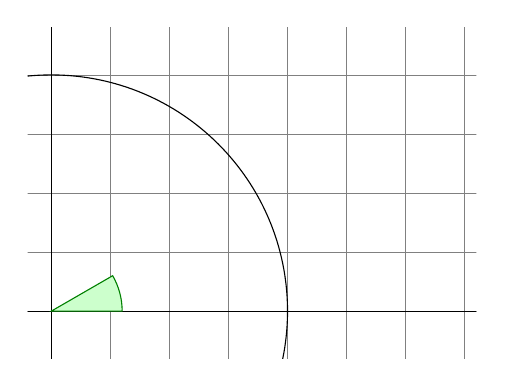
\begin{tikzpicture}[scale=3]
  \clip (-0.1,-0.2)
     rectangle (1.8,1.2);
  \draw[step=.25cm,gray,very thin]
       (-1.4,-1.4) grid (3.4,3.4);
  \draw (-1.5,0) -- (2.5,0);
  \draw (0,-1.5) -- (0,1.5);
  \draw (0,0) circle (1cm);
  \filldraw[fill=green!20!white,
            draw=green!50!black]
    (0,0) -- (3mm,0mm) 
         arc (0:30:3mm) -- cycle;
\end{tikzpicture}
\end{example}
Observe el carácter punto y coma (\texttt{;}). Separa los comandos individuales.

Un simple diagrama  de Venn
\begin{example}
\shorthandoff{:}
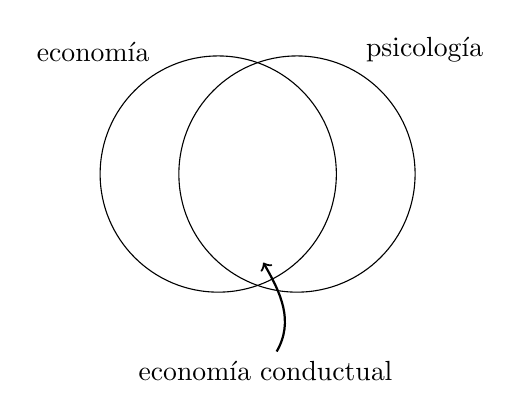
\begin{tikzpicture}
  \node[circle,draw,
        minimum size=3cm,
        label=120:{economía}]
         at (0,0) {};
  \node[circle,draw,
        minimum size=3cm,
        label=60:{psicología}]
         at (1,0) {};
  \node (i) at (0.5,-1) {};
  \node at (0.6,-2.5) 
    {economía conductual}
    edge[->,thick,
         out=60,in=-60] (i);
\end{tikzpicture}
\end{example}
Si está utilizando \pai{TikZ} en relación con \pai{babel} algunos de los caracteres utilizados en el lenguaje TikZ pueden ser modificados por \pai{babel}, lo que lleva a errores singulares. Para contrarrestar este problema, agregue el comando \ci{shorthandoff} a su código.

Observe los bucles foreach en el siguiente ejemplo.
\begin{example}
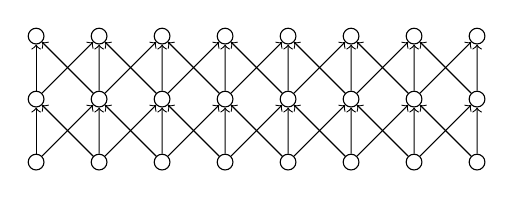
\begin{tikzpicture}[scale=0.8]
  \tikzstyle{v}=[circle, minimum size=2mm,inner sep=0pt,draw]
  \foreach \i in {1,...,8}
    \foreach \j in {1,...,3}
      \node[v] 
        (G-\i-\j) at (\i,\j) {};
  \foreach \i in {1,...,8}
    \foreach \j/\o in {1/2,2/3}
      \draw[->] 
        (G-\i-\j) -- (G-\i-\o);
  \foreach \i/\n in 
    {1/2,2/3,3/4,4/5,5/6,6/7,7/8}
    \foreach \j/\o in {1/2,2/3} {
       \draw[->] (G-\i-\j) -- (G-\n-\o);
       \draw[->] (G-\n-\j) -- (G-\i-\o);
    }
\end{tikzpicture}
\end{example}

Con la orden \ci{usetikzlibrary} en el preámbulo puede habilitar una amplia variedad de características adicionales para dibujar formas especiales, como esta caja que está ligeramente curvada.
\begin{example}
\usetikzlibrary{%
  decorations.pathmorphing}
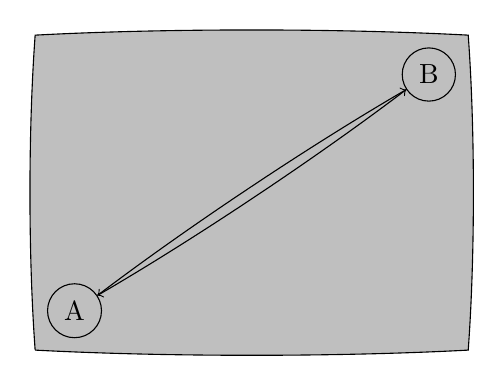
\begin{tikzpicture}[
     decoration={bent,aspect=.3}]
 \draw [decorate,fill=lightgray]
        (0,0) rectangle (5.5,4);
 \node[circle,draw] 
        (A) at (.5,.5) {A};
 \node[circle,draw] 
        (B) at (5,3.5) {B};
 \draw[->,decorate] (A) -- (B);
 \draw[->,decorate] (B) -- (A);
\end{tikzpicture}
\end{example}

\begin{example}
\usetikzlibrary{positioning}
\begin{tikzpicture}[xscale=6,
     yscale=8,>=stealth]
  \tikzstyle{v}=[circle,
     minimum size=1mm,draw,thick]
  \node[v] (a) {$1$};
  \node[v] (b) [right=of a] {$2$};
  \node[v] (c) [below=of a] {$2$};
  \node[v] (d) [below=of b] {$1$};
  \draw[thick,->] 
        (a) to node {} (c);
  \draw[thick,->] 
        (a) to node {} (d);
  \draw[thick,->] 
        (b) to node {} (d);
\end{tikzpicture}
\end{example}
 
 Incluso puede dibujar diagramas de sintaxis que se ven como si vinieran directamente de un libro sobre programación en Pascal. El código es un poco más intimidante que el ejemplo anterior, por lo que sólo mostraré el resultado. Si usted echa un vistazo en la documentación de \pai{pgf} encontrará un tutorial detallado sobre la elaboración de este diagrama exacto.

 \begin{center}
\begin{tikzpicture}[point/.style={coordinate},thick,draw=black!50,>=stealth',
                    tip/.style={->,shorten >=1pt},every join/.style={rounded corners},
                    skip loop/.style={to path={-- ++(0,#1) -| (\tikztotarget)}},
                    hv path/.style={to path={-| (\tikztotarget)}},
                    vh path/.style={to path={|- (\tikztotarget)}},
                 terminal/.style={
            rounded rectangle,
            minimum size=6mm,
            thick,draw=black!50,
            top color=white,bottom color=black!20,
            font=\ttfamily\tiny},
                nonterminal/.style={
                       rectangle,
                       minimum size=6mm,
                       thick,
                       draw=red!50!black!50,         % 50% red and 50% black,
                       top color=white,              % a shading that is white at the top...
                       bottom color=red!50!black!20, % and something else at the bottom
                       font=\itshape\tiny}]
\matrix[column sep=4mm] {
  % First row:
  & & & & & & & & & & & \node (plus) [terminal] {+};\\
  % Second row:
  \node (p1) [point] {}; &     \node (ui1)    [nonterminal] {entero sin signo}; &
  \node (p2) [point] {}; &     \node (dot)    [terminal]    {.};                &
  \node (p3) [point] {}; &     \node (digit) [terminal]     {dígito};            &
  \node (p4) [point] {}; &     \node (p5)     [point] {};                       &
  \node (p6) [point] {}; &     \node (e)      [terminal]    {E};                &
  \node (p7) [point] {}; &                                                      &
  \node (p8) [point] {}; &     \node (ui2)    [nonterminal] {entero sin signo}; &
  \node (p9) [point] {}; &     \node (p10)    [point]       {};\\
  % Third row:
  & & & & & & & & & & & \node (minus)[terminal] {-};\\
};
{ [start chain]
  \chainin (p1);
  \chainin (ui1)   [join=by tip];
  \chainin (p2)    [join];
  \chainin (dot)   [join=by tip];
  \chainin (p3)    [join];
  \chainin (digit) [join=by tip];
  \chainin (p4)    [join];
  { [start branch=digit loop]
    \chainin (p3) [join=by {skip loop=-6mm,tip}];
  }
  \chainin (p5)    [join,join=with p2 by {skip loop=6mm,tip}];
  \chainin (p6)    [join];
  \chainin (e)     [join=by tip];
  \chainin (p7)    [join];
  { [start branch=plus]
    \chainin (plus) [join=by {vh path,tip}];
    \chainin (p8)    [join=by {hv path,tip}];
  }
  { [start branch=minus]
    \chainin (minus) [join=by {vh path,tip}];
    \chainin (p8)    [join=by {hv path,tip}];
  }
  \chainin (p8)    [join];
  \chainin (ui2)   [join=by tip];
  \chainin (p9)    [join,join=with p6 by {skip loop=-11mm,tip}];
  \chainin (p10)   [join=by tip];
}
\end{tikzpicture}
\end{center}

Y hay más, si tiene que dibujar gráficas de datos o funciones numéricas, usted puede echar un vistazo más de cerca al paquete \pai{pgfplot}. Ofrece todo lo necesario para dibujar gráficos. Incluso puede llamar al comando externo \texttt{gnuplot} para evaluar las funciones reales que trazó en el gráfico.

Para una mayor inspiración, asegúrese de visitar la excelente página \linebreak \url{http://www.texample.net/tikz/} de Kjell Magne Fauske que contiene un depósito cada vez más grande de hermosos gráficos y otro tipo de código \LaTeX{}. En \TeX{}ample.net también encontrará una  \href{http://www.texample.net/tikz/resources/#tools-that-generate-pgftikz-code}{lista de herramientas} para trabajar con PGF/TikZ de modo que usted no tenga que escribir todo ese código a mano.

%%% Local Variables:
%%% TeX-master: "lshort.tex"
%%% mode: flyspell
%%% TeX-PDF-mode: t
%%% End: